% appendix_b
\chapter{Extension of an Empirically Driven Variability-Based Filtering Framework to Breast Tissue}
\label{app:empirical_variability_extension}

%-----------------------------------------------------------------------
\section{Motivation and Scope}
%-----------------------------------------------------------------------

The variability-based filtering strategy embedded in the preprocessing 
pipeline of this thesis builds directly on the method proposed 
by \cite{Edgar2017}, who demonstrated that a substantial fraction 
of CpG sites interrogated by the Illumina HumanMethylation450K array 
are effectively non-variable within a given tissue context and can 
therefore be removed prior to downstream analysis without loss of 
discriminative information. The original study was conducted on three 
healthy reference tissues — blood, buccal epithelial cells, and 
placenta — and the resulting non-variable CpG lists were shown to be 
robust across preprocessing pipelines and normalisation strategies.

The present appendix documents the extension of this framework to 
breast tissue. The extension pursues two objectives: (i) to assess 
whether the non-variability criterion, as originally defined, 
generalises to a cancer-relevant tissue under increased biological 
heterogeneity; and (ii) to provide a general, reproducible protocol 
for incorporating additional tissues into the reference framework 
in future studies. The analysis operates exclusively on 
histologically normal samples to preserve comparability with the 
original reference tissues and to estimate baseline methylation 
stability in the absence of disease-related confounding.
Importantly, this appendix does not modify the non-variability 
definition of \cite{Edgar2017}: a CpG is classified as non-variable 
if its inter-quantile range $r_{\beta,j} = Q_{0.90}(\beta_j) - 
Q_{0.10}(\beta_j) < 0.05$. The contribution is therefore evaluative and integrative rather than definitional.

%-----------------------------------------------------------------------
\section{General Framework for Cross-Tissue Extension}
\label{app:sec:framework}
%-----------------------------------------------------------------------

Let $\mathcal{T} = \{T_1, \dots, T_k\}$ denote a set of reference 
tissues, each represented by one or more independent methylation 
datasets from normal samples. For each tissue $T_\ell$, the 
tissue-specific non-variable CpG set is defined as:
\begin{equation}
    \mathcal{N}_\ell(\tau)
    =
    \left\{
    j \in \{1,\dots,p\} :
    Q_{0.90}\!\left(\beta_j^{(\ell)}\right)
    -
    Q_{0.10}\!\left(\beta_j^{(\ell)}\right)
    < \tau
    \right\},
    \label{eq:nv_tissue}
\end{equation}
where $\tau = 0.05$ is the threshold inherited from 
\cite{Edgar2017}. The cross-tissue invariant core — CpGs 
non-variable across all reference tissues simultaneously — is 
given by the intersection:
\begin{equation}
    \mathcal{N}_{\mathrm{core}}(\tau)
    =
    \bigcap_{\ell=1}^{k} \mathcal{N}_\ell(\tau).
    \label{eq:nv_core}
\end{equation}
When a new tissue $T_{k+1}$ is incorporated, the invariant 
core is updated as:
\begin{equation}
    \mathcal{N}_{\mathrm{core}}'(\tau)
    =
    \mathcal{N}_{\mathrm{core}}(\tau)
    \;\cap\;
    \mathcal{N}_{k+1}(\tau),
    \label{eq:nv_update}
\end{equation}
which is strictly more conservative than the original core: 
$\mathcal{N}_{\mathrm{core}}'(\tau) \subseteq 
\mathcal{N}_{\mathrm{core}}(\tau)$.
The validation of any extension requires verifying three 
properties before the updated core can be considered 
methodologically sound:
\begin{enumerate}
    \item \textbf{Selection stability}: the non-variable set 
    $\mathcal{N}_{k+1}(\tau)$ must be robust to dataset 
    composition, i.e.\ not driven by any single cohort 
    (Step~A, Section~\ref{app:sec:stepA}).
    \item \textbf{Threshold optimality}: the chosen $\tau$ 
    must lie at a favourable stability--dimensionality 
    trade-off point in the new tissue context 
    (Step~B, Section~\ref{app:sec:stepB}).
    \item \textbf{Empirical coherence}: the selected CpGs 
    must exhibit methylation and variability profiles 
    consistent with the non-variability interpretation, 
    ruling out selection artefacts 
    (Steps~C--D, Sections~\ref{app:sec:stepC}--\ref{app:sec:stepD}).
\end{enumerate}
This three-step validation protocol is general and applies 
identically to any future tissue extension.

%-----------------------------------------------------------------------
\section{Cross-Tissue Overlap Structure}
\label{app:sec:overlap}
%-----------------------------------------------------------------------

Breast tissue was introduced alongside the three original 
reference tissues of \cite{Edgar2017}. Figure~\ref{fig:point0_global_structure} 
reports the overlap structure of tissue-specific non-variable 
CpG sets across all four tissues.

\begin{figure}[t]
\centering
\begin{subfigure}[t]{0.48\textwidth}
  \centering
  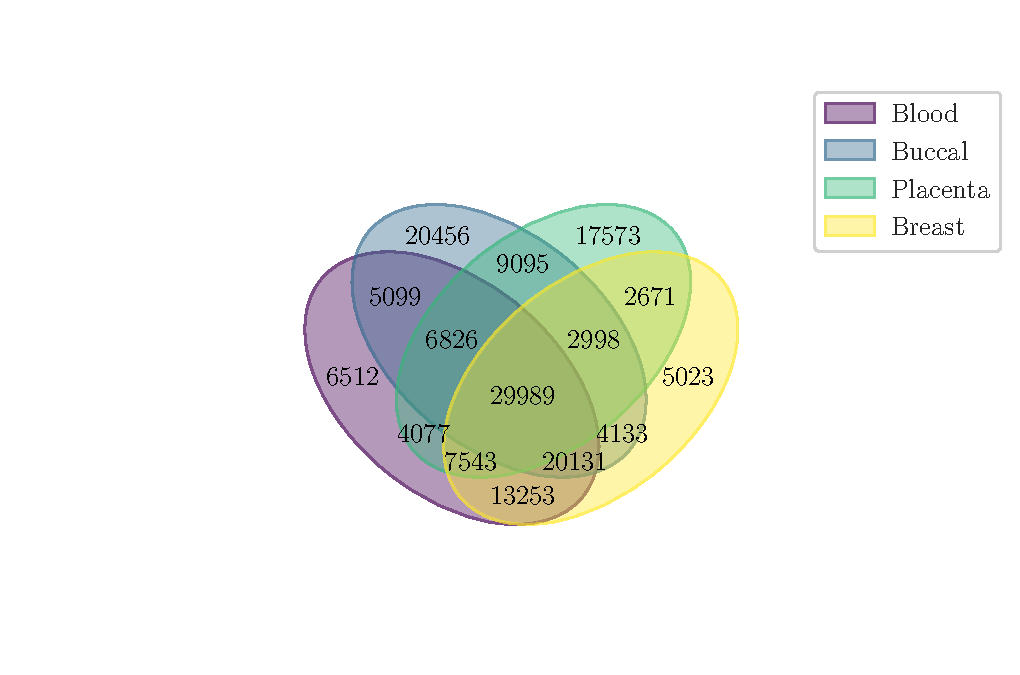
\includegraphics[width=\textwidth]{images/appendix/venn_4tissues_invariants.pdf}
  \caption{Pairwise and higher-order overlaps of tissue-specific 
  non-variable CpG sets.}
\end{subfigure}
\hfill
\begin{subfigure}[t]{0.48\textwidth}
  \centering
  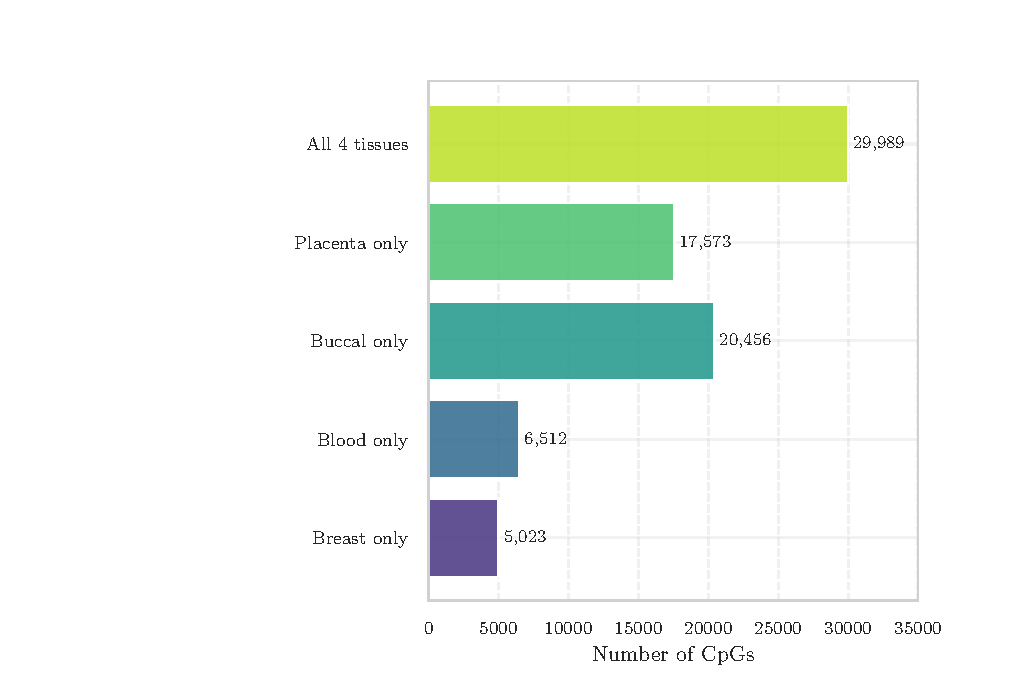
\includegraphics[width=\textwidth]{images/appendix/barplot_key_intersections_invariants.pdf}
  \caption{Quantitative intersection sizes for key subsets.}
\end{subfigure}
\caption{Global overlap structure of non-variable CpGs across 
blood, buccal epithelial cells, placenta, and breast tissue. 
}
\label{fig:point0_global_structure}
\end{figure}
The four-way invariant core $\mathcal{N}_{\mathrm{core}}'(0.05)$ 
comprises 29,989 CpGs — a substantial shared subset whose 
persistence despite the inclusion of a cancer-relevant tissue 
suggests that at least a component of CpG non-variability reflects stable, context-independent properties of the methylation 
landscape rather than purely tissue-specific regulatory 
programmes. The breast-exclusive non-variable set (5,023 CpGs) 
is the smallest tissue-specific component, consistent with the 
expectation that breast tissue introduces additional 
heterogeneity relative to the original healthy tissue panel.

%-----------------------------------------------------------------------
\subsection{Step A: Stability of Non-Variable CpG Selection}
\label{app:sec:stepA}
%-----------------------------------------------------------------------

The first validation step assesses whether the breast-tissue 
non-variable set $\mathcal{N}_{\mathrm{breast}}(\tau)$ is 
robust to dataset composition. A leave-one-dataset-out (LODO) 
strategy is adopted: for each held-out dataset 
$\mathcal{D}^{(-s)}$, the non-variable set is recomputed on 
the remaining datasets and compared to the full-reference set 
via the retention rate:
\begin{equation}
    \rho^{(-s)}
    =
    \frac{
        \left|\mathcal{N}_{\mathrm{breast}}^{(-s)}(\tau)
        \cap
        \mathcal{N}_{\mathrm{breast}}(\tau)\right|
    }{
        \left|\mathcal{N}_{\mathrm{breast}}(\tau)\right|
    },
    \label{eq:retention}
\end{equation}
where $\mathcal{N}_{\mathrm{breast}}^{(-s)}(\tau)$ denotes 
the non-variable set estimated without dataset $s$.
\begin{figure}[t]
\centering
\begin{subfigure}[t]{0.48\textwidth}
  \centering
  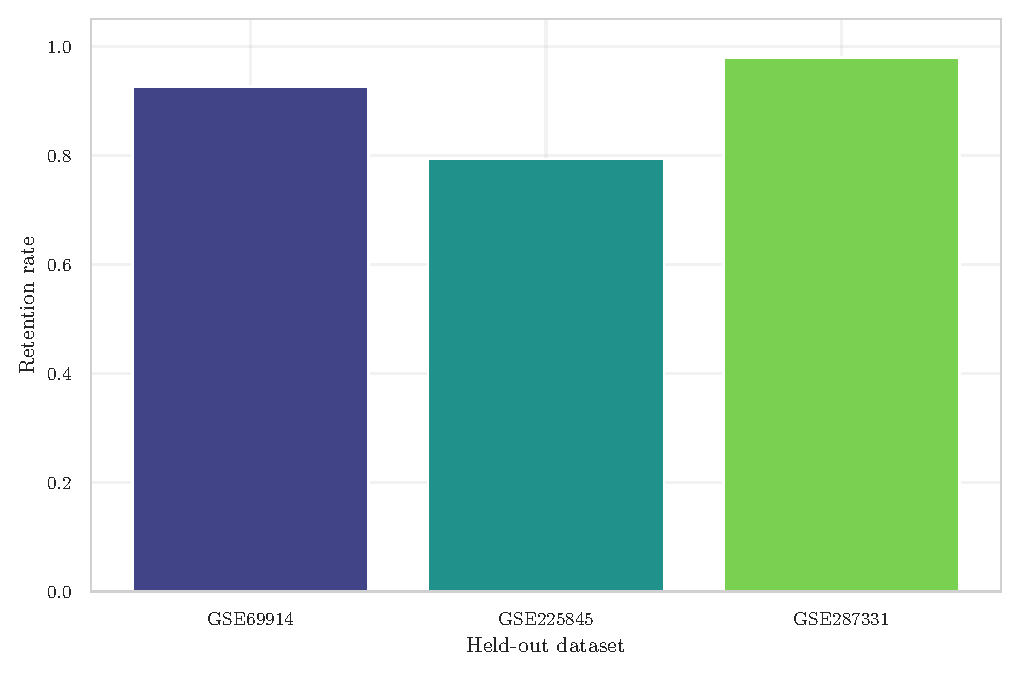
\includegraphics[width=\textwidth]{images/appendix/stepA_lodo_stability.pdf}
  \caption{Retention rates under the LODO protocol across 
held-out datasets (GSE69914, GSE225845, GSE287331).}
  \label{fig:stepA_lodo}
\end{subfigure}
\hfill
\begin{subfigure}[t]{0.48\textwidth}
  \centering
  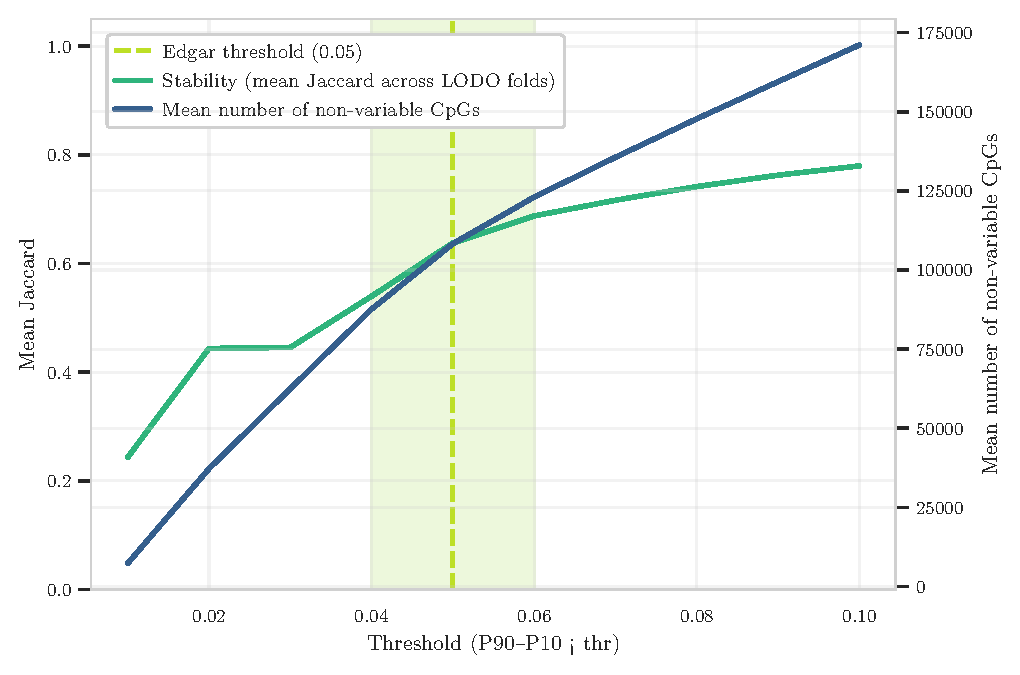
\includegraphics[width=\textwidth]{images/appendix/stepB_stability_vs_list_size_highlighted.pdf}
  \caption{Mean Jaccard similarity $J(\tau)$ and mean 
non-variable CpG count as functions of the threshold.}
  \label{fig:stepB_stability_vs_size}
\end{subfigure}

\caption{Assessment of robustness and trade-off between stability and dimensionality of non-variable CpG sets.}
\label{fig:stepAB}
\end{figure}
The retention rates reported in Figure~\ref{fig:stepA_lodo} 
are consistently high across all three held-out datasets, 
demonstrating that $\mathcal{N}_{\mathrm{breast}}(\tau)$ 
is not an artefact of any individual cohort but reflects 
a stable property of the underlying methylation variability 
structure in breast tissue. This result satisfies the first 
validation criterion stated in Section~\ref{app:sec:framework} 
and is a necessary condition for interpreting non-variability 
as a genuine empirical property rather than a dataset-specific 
anomaly.

%-----------------------------------------------------------------------
\subsection{Step B: Stability--Dimensionality Trade-Off}
\label{app:sec:stepB}
%-----------------------------------------------------------------------

Having established stability at $\tau = 0.05$, Step~B 
evaluates whether this threshold represents an optimal 
compromise between selection reproducibility and 
dimensionality reduction in the breast tissue setting. 
The mean Jaccard similarity across LODO folds and the 
mean number of non-variable CpGs are computed as 
functions of $\tau \in [0.01, 0.10]$:
\begin{equation}
    J(\tau)
    =
    \frac{1}{S}
    \sum_{s=1}^{S}
    \frac{
        \left|\mathcal{N}_{\mathrm{breast}}^{(-s)}(\tau)
        \cap
        \mathcal{N}_{\mathrm{breast}}(\tau)\right|
    }{
        \left|\mathcal{N}_{\mathrm{breast}}^{(-s)}(\tau)
        \cup
        \mathcal{N}_{\mathrm{breast}}(\tau)\right|
    }.
    \label{eq:jaccard}
\end{equation}
As shown in Figure~\ref{fig:stepB_stability_vs_size}, 
$J(\tau)$ increases rapidly for small $\tau$ and 
saturates before the Edgar threshold, while the CpG 
count continues to grow approximately linearly. 
At $\tau = 0.05$, stability is already at its 
near-maximum value and the marginal gain from 
increasing the threshold further is negligible relative 
to the dimensionality cost incurred. This empirically 
validates the original threshold of \cite{Edgar2017} 
in the breast tissue context and provides a 
data-driven justification for its retention within 
the extended framework.

%-----------------------------------------------------------------------
\subsection{Step C: Methylation Distribution of Non-Variable CpGs}
\label{app:sec:stepC}
%-----------------------------------------------------------------------

Step~C characterises the methylation profiles of the 
selected non-variable CpGs by comparing their 
$\beta$-value distribution to a random background 
sample of array CpGs, computed on normal breast 
samples pooled across datasets.
\begin{figure}[t]
\centering
\begin{subfigure}[t]{0.48\textwidth}
  \centering
  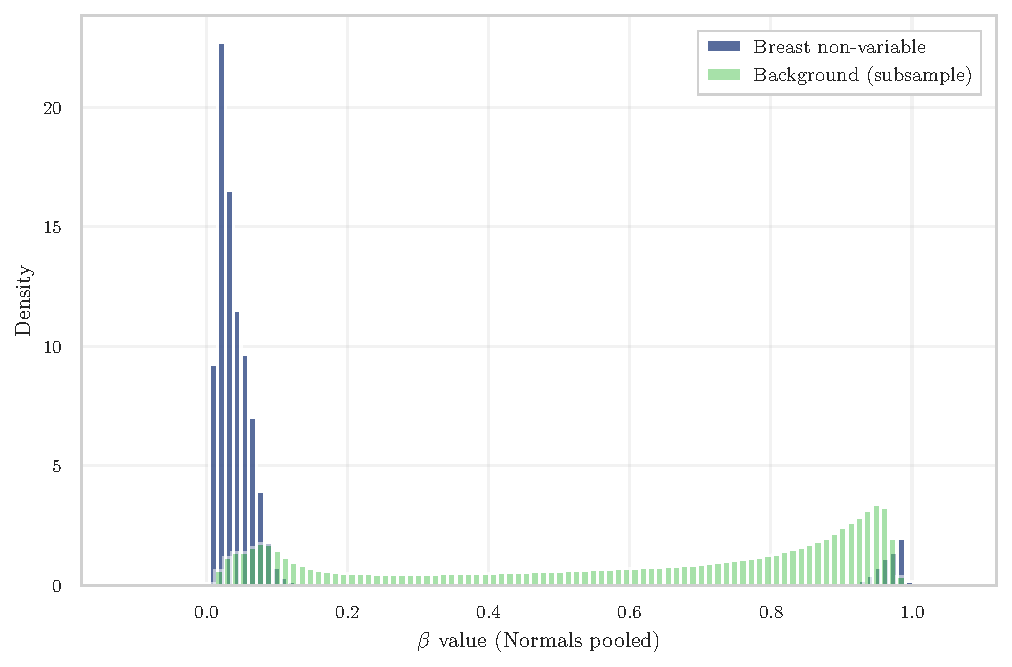
\includegraphics[width=\textwidth]{images/appendix/stepC_beta_distribution_nv_vs_background.pdf}
  \caption{Beta-value density for non-variable CpGs 
(breast tissue) versus genomic background.}
  \label{fig:stepC_beta_distribution}
\end{subfigure}
\hfill
\begin{subfigure}[t]{0.48\textwidth}
  \centering
  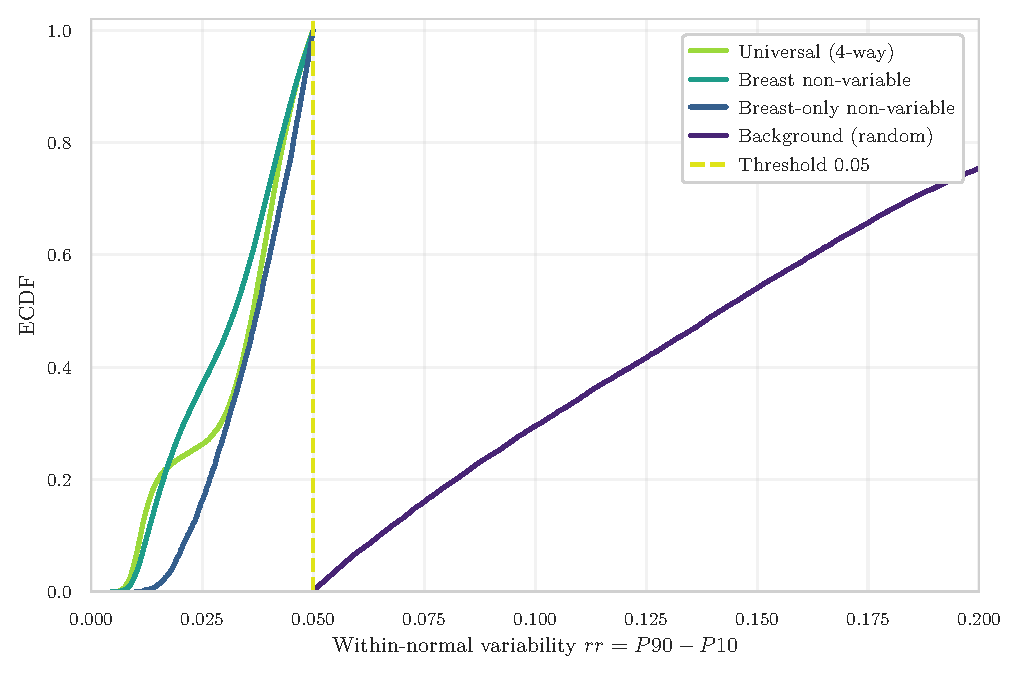
\includegraphics[width=\textwidth]{images/appendix/stepD_baseline_rr_ecdf.pdf}
  \caption{ECDF of within-normal variability 
$r_{\beta,j} = Q_{0.90} - Q_{0.10}$ across CpG subsets.}
  \label{fig:stepD_rr_ecdf}
\end{subfigure}

\caption{Characterization of the selected non-variable CpG set in terms of methylation distribution and baseline risk behavior.}
\label{fig:stepCD}
\end{figure}
Non-variable CpGs in breast tissue are strongly 
concentrated at extreme $\beta$ values, consistent 
with constitutive hypo- or hypermethylated states. 
This pattern replicates the findings of \cite{Edgar2017} 
in healthy tissues and extends them to a cancer-relevant 
context, supporting the interpretation that 
non-variability reflects stable regulatory configurations 
rather than artefacts of tissue composition or 
disease-related heterogeneity. The enrichment of 
non-variable CpGs in CpG islands and constitutively 
silenced promoter regions, documented in the original 
study, is consistent with this bimodal profile 
\cite{Edgar2017, Bock2012}.

%-----------------------------------------------------------------------
\subsection{Step D: Baseline Variability Profile}
\label{app:sec:stepD}
%-----------------------------------------------------------------------

Step~D provides quantitative validation of the filtering 
criterion by examining the empirical cumulative distribution 
function (ECDF) of $r_{\beta,j}$ across four CpG subsets: 
the four-way shared non-variable core 
$\mathcal{N}_{\mathrm{core}}'(0.05)$, the breast-specific 
non-variable set $\mathcal{N}_{\mathrm{breast}}(0.05)$, 
the breast-exclusive component, and a random background set.
The ECDFs in Figure~\ref{fig:stepD_rr_ecdf} show a 
clear separation: the non-variable subsets are sharply 
concentrated at low $r_{\beta,j}$ values, with the 
majority of CpGs well below $\tau = 0.05$, whereas 
the background distribution spans a substantially 
wider range. This confirms that the selected CpGs 
are empirically distinct in their variability profile 
and not merely defined as non-variable by construction. 
The consistency of this pattern across all non-variable 
subsets — including the breast-exclusive component — 
further supports the robustness of the extended 
framework.

%-----------------------------------------------------------------------
\section{Positioning Within the Thesis and Generalisability}
\label{app:sec:positioning}
%-----------------------------------------------------------------------

The extended framework described in this appendix 
provides the empirical grounding for the variability 
filter applied in Chapter~\ref{chap:feature_selection}. 
The four validation steps collectively establish that 
the non-variability criterion of \cite{Edgar2017} 
is stable, threshold-optimal, and biologically 
coherent when applied to breast tissue — necessary 
conditions for its use as a preprocessing step in 
the present study.

In the current analysis, datasets are processed 
independently and the non-variability threshold is 
estimated within each cohort separately, rather than 
enforcing a single shared CpG list across datasets. 
This design preserves dataset-specific methylation 
structure and avoids premature cross-cohort 
harmonisation, while the validation performed here 
ensures that the filtering criterion rests on 
population-level properties rather than 
cohort-specific artefacts.

The general framework formalised in 
Section~\ref{app:sec:framework} — update rule 
(Equation~\ref{eq:nv_update}), LODO stability 
assessment (Equation~\ref{eq:retention}), and 
Jaccard-based threshold analysis (Equation~\ref{eq:jaccard}) — 
is structurally independent of tissue type and 
platform density. It therefore remains applicable 
to future tissue extensions and to higher-density 
arrays such as the Illumina EPIC platform, whose 
expanded CpG coverage approximately doubles that 
of the 450K array \cite{Pidsley2016}.
